\documentclass[10pt]{article}

\usepackage{amsmath}% http://ctan.org/pkg/amsmath
\usepackage{amsthm}
\usepackage{todonotes}
\usepackage[margin=1in]{geometry}
\usepackage{algorithm}
\usepackage{url}
\usepackage[noend]{algpseudocode}
\usepackage{mdframed}
\usepackage{tikz}
\usetikzlibrary{matrix,shapes,arrows,positioning,chains, calc}

%% defining new theorem environment for definition
\newtheorem{defn}{\textbf{Definition}}
\newtheorem{thm}{\textbf{Theorem}}
\newtheorem{cor}{\textbf{Corollary}}
\newtheorem{lemma}{\textbf{Lemma}}

\renewcommand{\algorithmicrequire}{\textbf{Input:}}
\renewcommand{\algorithmicensure}{\textbf{Output:}}

\begin{document}
\title{{\sf AND\=aNA-v2}: Application-Layer Support for \\ Low-Latency Bidirectional Anonymous Traffic in NDN}
\author{Christopher A. Wood \\ UC Irvine \\ {\tt woodc1@uci.edu}}
\date{\today}
%\thanks{TODO}
\maketitle

%%% ABSTRACT
\begin{abstract}
This report documents the motivation, design, and implementation plan for the new version of {\sf AND\=aNA} to support highly efficient bidrectional traffic with low-latency in NDN. Weeks 1-3 of this project were spent setting up the experimental testbed and ramping up with the {\sf AND\=aNA} design and source code; weeks 4-6 were spent designing and running experiments to gather performance data for {\sf AND\=aNA}; weeks 7-8 were spent on the design of {\sf AND\=aNA-v2} and preliminary attempts at its implementation; weeks 9-10 were spent finalizing the design, completing the implementation, and gathering experimental data that can be used to compare against {\sf AND\=aNA}.
\end{abstract}

%%%%%%%%%%%%%%%%%%%%%
%%% MAIN CONTENT
%%%%%%%%%%%%%%%%%%%%%

\section{Overview} \label{sec:overview}
With the possibile adoption of NDN or any flavor of information-centric networking as the future Internet architecture in the near future, support for low-latency, bidirectional traffic may prove very useful for a variety of use cases. Consider the scenario in which two parties wish to exchange voice or video content over NDN, such as the case with Skype and related applications. Jacobson et al. \cite{voccn} have already studied the efficiencies of such content-heavy and QoS-strict applications over CCN. Unfortunately, support for such applications becomes much more difficult when one, or both, of the parties wishes to remain anonymous. Such is the case in settings where voice or video content is being streamed from \emph{some} person in a single organization, but the identity of said person needs to remain secret. A real-world instance where this may be useful is when such traffic needs to be exchanged between military organizations of unfriendly nations. Indeed, the identity of military personell participating in such voice or video conferences should remain secret for safety reasons. 

Application-layer support for anonymizing network traffic has already been implemented in the {\sf AND\=aNA} system \cite{andana}. However, in that work, the authors focus on a single, unidirectional client-producer scenario in which traffic latency, network jitter, and quality-of-service requirements were not specified nor mandated. In this work, we seek to amend the design of {\sf AND\=aNA} to support low-latency, bidrectional traffic applications with hard QoS and anonymity requirements. Consequently, this new design seeks to attain equivalent anonymity and privacy guarantees of {\sf AND\=aNA} while enjoying significantly higher performance - two factors that are often inversely related in practice. 

In the remainder of this document we discuss the motivation and details of our preliminary design for the new anonymizing application, dubbed {\sf AND\=aNA-v2}, as well as our implementation strategy. In order to avoid confusion and repetition throughout the rest of the document, all common terminology used throughout is specified and clarified in Table \ref{tab:notation}. Also, for simplicity, we denote the global system security parameter as $\kappa$, unless otherwise specified. 

\begin{table}
\centering
\caption{Notation used in the presentation of this work.}
\label{tab:notation}
  \begin{tabular}{| r | l |} \hline
  $\mathsf{C}$ & Set of all consumers  \\
  $\mathsf{P}$ & Set of all producers  \\ 
  $\mathsf{R}$ & Set of all routers  \\
  $\mathsf{IF}$ & Set of all interfaces on all routers  \\
  $\mathsf{if}_i^r \in \mathsf{IF}$ & Interface $i$ of router $r$  \\
  $(pk_i, sk_i)$ & Public/private key pair for router $r$  \\
  $\overline{\mathsf{int}}_{i}^{j}$ & Encrypted interest wrapped from router $i$ to router $j$ ($i \leq j$)  \\
  $\mathcal{A}$ & Adversary \\ 
  $u$ & Entity in the network (consumer or producer) \\
  $u \to_{\mathsf{int}} r$ & Entity $u$ sends interest to router $r$  \\ 
  $\mathsf{int} \to \mathsf{if}_i^r$ & Interest $\mathsf{int}$ is sent to interface $i$ of router $r$ \\
  $r \in \mathsf{R}$ & An anonymizing router (AR) \\ 
  $\mathcal{E}_{pk_i}(\cdot)$ & Public key encryption using $pk_i$ \\ 
  $\mathcal{D}_{pk_i}(\cdot)$ & Public key decryption using $pk_i$ \\ 
  $\mathsf{Encrypt}_{k_i}(\cdot)$ & Symmetric key encryption using key $k_i$ \\ 
  $\mathsf{Decrypt}_{k_i}(\cdot)$ & Symmetric key decrypt using key $k_i$ \\ 
  $\mathsf{ST}$ & AR session table used to store session ID and digest tuples \\
  $H$ & A collision resistant hash function on the domain $\{0,1\}^*$ to range $\{0,1\}^{\kappa}$ \\
  $F_k$ & A keyed pseudorandom function \\ \hline
  \end{tabular}
\end{table}

\section{Motivation}
The primary motivation for a new desgin of {\sf AND\=aNA} is to attain the same anonymity and privacy guarantees as {\sf AND\=aNA} with \emph{better} performance. The original design targeted a single use case in which performance, especially in the bidirectional setting, was not a primary concern. Indeed, there was both an asymmetric and symmetric (session-based) variant of {\sf AND\=aNA}, and while the latter enjoyed better speedups over the former it suffered the fatal flaw of not ensuring packet unlinkability. It is generally the case that unlinkability is merely sufficient for anonymity, rather than also being a necessary condition for anonymity. However, in the case of {\sf AND\=aNA}, packet linkability can lead to consumer and producer linkability, which immediately violates anonymity. For example, it is not difficult to hypothesize an adversary that eavesdrops on incoming and outgoing interests for a particular anonymous router, and who by doing so is able to determine that the incoming and outgoing session IDs are linked. In fact, a modified type of this kind of adversary was explicitly studied in the context of Tor by Murdoch and Danezis in \cite{tor-traffic-analysis}. In their work, the goal of the adversary in their ``linkability attack'' was to determine whether two separate data streams being served by two corrupted servers were initiated by the same consumer, and we suspect that such analysis could be augmented to work for {\sf AND\=aNA}. Specifically, repeating a packet linkability attack at each anonymous router in a circuit may therefore eventually lead to linkability between the producer and consumer. The use of application and environment contextual information has also been formally studied in \cite{attacking-unlinkability}, in which side channel and environment information (e.g., the deterministic behavior of an anonymous router always forwarding a packet upstead after unwrapping an interest received from some downstream router) is used to quantify the \emph{degree of unlinkability}. Furthermore, we remark that regardless of how such linkability information is acquired, it has been shown that it can lead to reduce consumer and producer anonymity beyond what is possible with general traffic analysis \cite{linkability-attacks}. 

As most of the literature focuses on mix-based anonymizing services like Tor, which inspired the original design of {\sf AND\=aNA}, it is clear that any form of linkability should be avoided in order to maintain consumer and producer anonymity. Therefore, the formal goal for {\sf AND\=aNA-v2} is to attain the same anonymity and privacy guarantees as the asymmetric variant of {\sf AND\=aNA}, which does not suffer from packet linkability issues, while supporting high-throughput and low-latency traffic between two parties. 

% TODO: need for more performance and better security (problems with ANDNAv1, what we can do better, why unlinkability is a bad thing - cite related work here)

\section{Circuit and Session Establishment}
At the heart of the {\sf AND\=aNA} is the notion of anonymizing routers and connection-oriented circuits, similar in spirit to the inner workings of TOR \cite{tor}. Anonymizing routers serve two purposes in {\sf AND\=aNA}: (1) to decapsulate and forward encrypted interests, along with content encryption keys, generated by a consumer until the cleartext interest arrives at the producer, and (2) to encapsulate sensitive content using the previously acquired encryption keys and relay the encrypted content downstream. In this way, the consumer generates an interest wrapped by several layers of encryption and receives a piece of content wrapped in several layers of encryption that it can easily decrypt. It is also important to note that since each anonymizing router operates at the application layer, it effectively serves as the producer for each downstream router in the {\sf AND\=aNA} circuit. Therefore, NDN policy dictates that such content \emph{must be signed}. Verification of content from upstream routers, however, is not mandatory. 

We also note that the current {\sf AND\=aNA} design has support for two types of circuits: asymmetric and symmetric session-based. In the asymmetric variant, all encrypted interests are done using a CCA-secure PKI scheme and all content is encrypted using a CCA-secure symmetric key encryption scheme. Conversely, in the session-based variant, all encrypted interests are protected using a CCA-secure symmetric key encryption scheme, where the key is identified using a unique session identifier sent in the cleartext along with the encrypted interests. This worsens anonymity because it provides a way to link packets to a single session (as previously discussed).

Putting together all of the design aspects of the current version of {\sf AND\=aNA}, we see that the following factors weigh in on the overall performance of the application:
\begin{enumerate}
  \item Content encryption
  \item Content signature generation
  \item Encrypted interest generation
\end{enumerate} 
In {\sf AND\=aNA-v2} we seek to minimize the degree to which these factors affect interest and content encapsulation and decapsulation by integrating support for anonymous router \emph{state}, which is encapsulated in sessions, into anonymous circuits. Sessions will exist for unidirectional traffic only, which therefore means that bidirection traffic, the ultimate focus of this work, will require two sessions to be established and maintained for the duration of the bidirectional application. This is done so that each party in the application need not use the same set of anonymous routers for communication. Not only does this free each consumer to select a random subset of anonymous routers $r_1,r_2,\dots,r_n$ from the set of total anonymous routers $\mathsf{R}$, but it may also help improve QoS guarantees by distributing the load of encapsulation and decapsulation among multiple nodes. Furthermore, sessions enable the establishment of long-term secrets that can be used to improve the efficiency of certain cryptographic operations, such as content encryption, signature generation, and signature verification. 

With the end of goal of supporting highly efficient and anonymous bidirectional traffic, the goals of the circuit and session establishment using a list of $n$ anonymous routers $r_1,\dots,r_n$ are as follows:
\begin{enumerate}
\item Establish unique session IDs $\mathsf{session}_{i}$ and session IVs $\mathsf{SIV}_i$
\item Establish content encryption keys $E_{k_i}$ and initial counter values $\mathsf{EIV}_i$
\item Establish pairwise MAC keys $M_{k_i}$ used to sign (and optionally verify) content
\end{enumerate}
The purpose of each of these session entities will become clear from the circuit initialization and usage procedures. After establishment, the circuit from the consumer $C$ to the producer $P$ should be similar to that shown in Figure \ref{fig:circuit}. We now describe the general protocol for establishing this type of session-based circuit from a consumer $C$ to a producer $P$ given $n$ anonymous routers. Recall that, in order to support bidirectional communication, $P$ would have to establish a similar circuit to $C$ with $m$ routers, where $m$ need not equal $n$. 
\begin{algorithm}[ht!]
  \caption{Circuit and Session Establishment Protocol}
  \begin{algorithmic}[1]
    \Require{Anonymous routers $r_1,r_2,\dots,r_n$ ($n \geq 2$) with public keys $pk_1,pk_2,\dots,pk_n$.}

\Function{{\sf ServerRetrieveMACKey}}{$\mathsf{int}$} // Server-side at router $i$
  \State $(M_{k}, \mathsf{session}_i, x) := \mathcal{D}_{sk_i}(\mathsf{int}[-1])$ // Recover MAC key and randomness $x$
  \If{$\mathsf{session}_i$ not in state}
    \State \Return $\mathsf{Error}$
  \Else
    \State Persist $M_k$ as $M_{k_{i+1}}$ (the upstream MAC key) with session $\mathsf{session}_i$
    \State $x^* := \mathsf{MAC}_{M_{k}}(x)$
    \State $\mathsf{resp} := x^*$
    \State \Return $\mathsf{resp}$
  \EndIf

  % \State $(E_{k_n}, M_{k_n}, \mathsf{EIV}_n, \mathsf{session}_n, \mathsf{SIV}_n) \gets \overline{\mathcal{D}_{k}}(T)$
  % \State \Return $(E_{k_n}, M_{k_n}, c_n, \mathsf{session}_n, \mathsf{IV}_n)$
\EndFunction

\Function{{\sf ServerEstablishSession}}{$\mathsf{int}$} // Server-side at router $i$
  \State $k \gets \mathcal{D}_{sk_i}(\mathsf{int}[-1])$ // Recover session encryption key
  \State $E_{k_i} \gets \{0,1\}^{\kappa}$ // Encryption key
  \State $M_{k_i} \gets \{0,1\}^{\kappa}$ // MAC key
  \State $\mathsf{EIV}_i \gets \{0,1\}^{\kappa}$     // counter IV
  \State $x \gets \{0,1\}^{\kappa}$
  \State $\mathsf{SIV}_i \gets \{0,1\}^{\kappa}$ // session IV
  \State $\mathsf{session}_i := H(x)$ // session ID
  \State $\mathsf{SIndex}_i := H(\mathsf{session}_i + \mathsf{SIV}_i)$
  \State Persist $(\mathsf{session}_i, E_{k_i}, M_{k_i}, \mathsf{EIV}_i, \mathsf{SIV}_i)$ to state, and store $(\mathsf{SIndex}_i, \mathsf{session}_i, \mathsf{SIV}_i)$ in the session table $\mathsf{ST}_i$
  \State $\mathsf{resp} \gets \mathsf{Encrypt}_{k}(\mathsf{session}_i, E_{k_i}, M_{k_i}, \mathsf{EIV}_i, \mathsf{SIV}_i)$
  \State \Return $\mathsf{resp}$
  
  % \State $T' := \mathcal{D}_{sk}(T)$ // Secret key $sk$ corresponding to the receiving router $r$
  % \If {$|T'| = 4$}
  %   \State Persist $(\mathsf{session}, E_{k}, c, M_{k})$ to state
  % \Else
  %   \State Persist $(\mathsf{session}, E_{k}, c, M_{k}, M_{k_{+1}})$ to state
  % \EndIf
\EndFunction

\Function{{\sf ClientSendMACKey}}{$r_i$, $\mathsf{session}_i$, $M_{k}$} // Client-side
  \State $x \gets \{0,1\}^{\kappa}$
  \State $x' := \mathsf{MAC}_{M_{k}}(x)$
  \State $T \gets \mathcal{E}_{pk_i}(M_{k}, \mathsf{session}_i, x)$
  \State $\mathsf{int} := \mathsf{namespace}_i/\mathsf{SESSIONMAC}/T$
  \State $\mathsf{resp} := \mathsf{ccnget}(\mathsf{int})$ // reach out to the AR
  \State $x^* := \mathsf{resp}[-1]$
  \If{$x' \not= x^*$}
    \State \Return $\mathsf{Fail}$
  \Else
    \State \Return $\mathsf{Pass}$
  \EndIf

  % \State $(E_{k_n}, M_{k_n}, \mathsf{EIV}_n, \mathsf{session}_n, \mathsf{SIV}_n) \gets \overline{\mathcal{D}_{k}}(T)$
  % \State \Return $(E_{k_n}, M_{k_n}, c_n, \mathsf{session}_n, \mathsf{IV}_n)$
\EndFunction

\Function{{\sf ClientEstablishSession}}{$r_i$} // Client-side
  \State $k \gets \{0,1\}^{\kappa}$
  \State $\overline{k} \gets \mathcal{E}_{pk_i}(k)$
  \State $\mathsf{int} := \mathsf{namespace}_i/\mathsf{CREATESESSION}/\overline{k}$
  \State $\mathsf{resp} := \mathsf{ccnget}(\mathsf{int})$ // reach out to the AR
  \State $(E_{k_n}, M_{k_n}, \mathsf{EIV}_n, \mathsf{session}_n, \mathsf{SIV}_n) \gets \mathsf{Decrypt}_{k}(\mathsf{resp})$
  \State \Return $(E_{k_n}, M_{k_n}, c_n, \mathsf{session}_n, \mathsf{IV}_n)$
\EndFunction

% \State $E_{k_i} \gets \{0,1\}^k$ for $k = 1,\dots,n$ // Encryption key
% \State $M_{k_i} \gets \{0,1\}^k$ for $k = 1,\dots,n$ // MAC key
% \State $c_i \gets \{0,1\}^k$ for $k = 1,\dots,n$     // counter IV
% \State $x \gets \{0,1\}^k$
% \State $\mathsf{session}_n := H(x)$
% \State $T' := (\mathsf{session}_n, E_{k_n}, c_n, M_{k_n})$
% \State $T_n := \mathcal{E}_{pk_n}(T')$

\Function{{\sf EstablishCircuit}}{$r_1,\dots,r_n$} // Main procedure
\State $(E_{k_n}, M_{k_n}, c_n, \mathsf{session}_n, \mathsf{IV}_n) := \mathsf{ClientEstablishSession}(r_n)$
\For{$i = n - 1$ \textbf{ downto } $1$}
  \State $(E_{k_i}, M_{k_i}, \mathsf{EIV}_i, \mathsf{session}_i, \mathsf{SIV}_i) := \mathsf{ClientEstablishSession}(r_n)$
  \If{$\mathsf{ClientSendMACKey}(r_i, \mathsf{session}_i, M_{k_{i+1}}) = \mathsf{Fail}$}
    \State \Return $\mathsf{Fail}$
  \EndIf
  % \State $\mathsf{session}_{i} := H(\mathsf{session}_n \bigoplus_{j=i}^{n} E_{k_j})$
  % \State $T' := (\mathsf{session}_i, E_{k_i}, c_i, M_{k_i}, M_{k_{i+1}})$
  % \State $T_n := \mathcal{E}_{pk_i}(T_i)$
  % \State $\mathsf{EstablishSession}(T_i)$
\EndFor
\EndFunction

  \end{algorithmic}
\end{algorithm}

Notice that by this procedure, no two routers will share the same session identifier even though they partake in the same circuit since they generate session identifiers independent and uniformly at random from $\{0,1\}^{\kappa}$. Also, the {\sf ServerEstablishSession} and {\sf ServerRetrieveMACKey} procedures are asynchronous and only invoked in response to the respective interest.

\begin{figure}[ht!]
\begin{center}
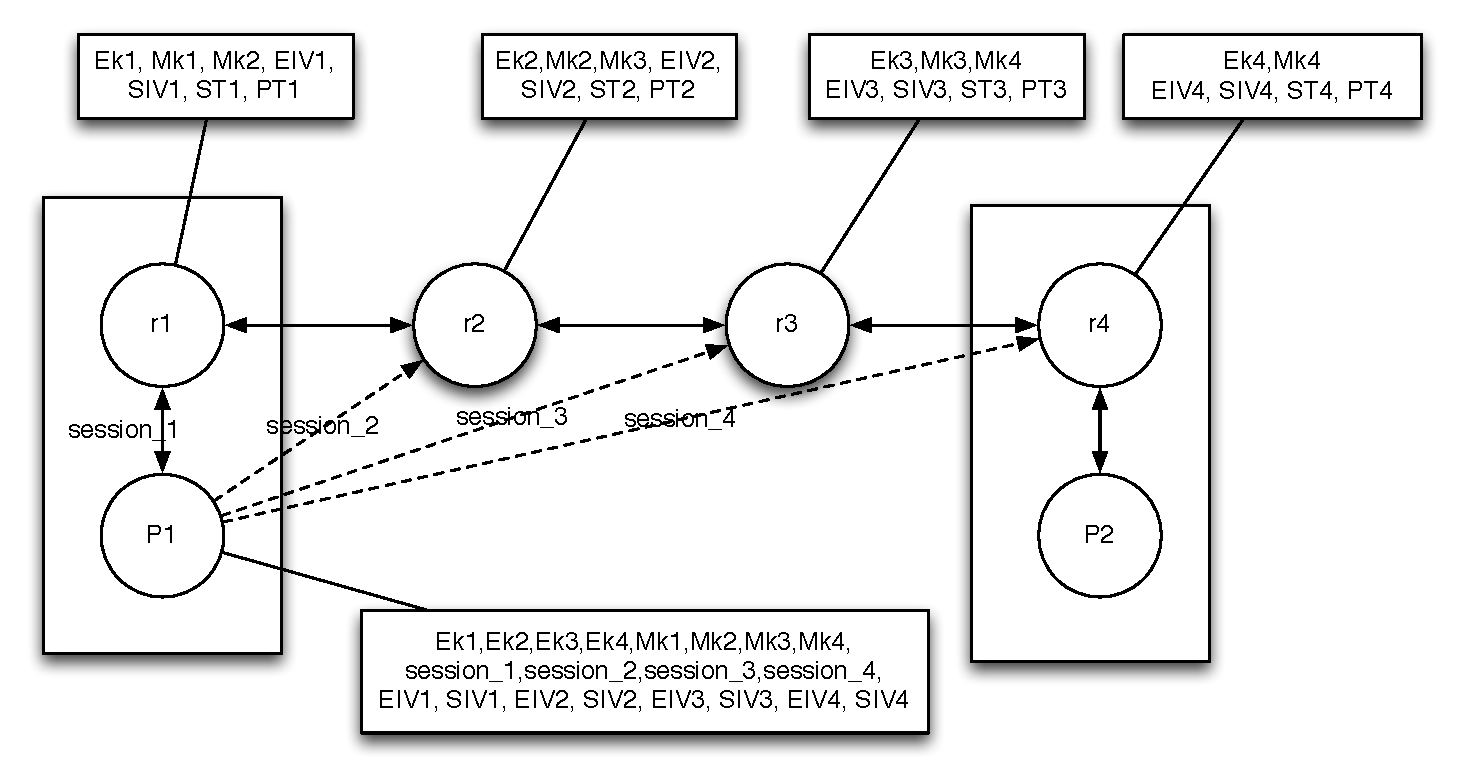
\includegraphics[scale=0.5]{./images/circuit.pdf}
\end{center}
\caption{Sample session-based circuit between a consumer $C$ and producer $P$ with ARs $r_1,r_2,r_3,r_4$, where the end routers on the path are run on the same node as $C$ and $P$.}
\label{fig:circuit}
\end{figure}

\subsection{{\sf AND\=aNA-v2} Circuit Usage}

We note that anonymous routers must be chosen in a \emph{mutually excluse} manner, meaning that they do not change share the same name prefix or are from the same organization (see Figure \ref{fig:pool}). This requirement is needed for ensuring anonymity. After a circuit and the corresponding sessions have been created between the consumer and each anonymous router, usage of the circuit proceeds as per the original {\sf AND\=aNA} design. Specifically, there are three main operations that need to be defined: encrypted interest generation, AR interest forwarding, and AR content handling. In what we follows we present the details of each of these procedures as needed for {\sf AND\=aNA-v2}. We begin with the encrypted interest generation procedure (shown in Algorithm \ref{alg:enc_int_gen}) in which a consumer $C$ particpating in a particular \emph{application} session with a producer $P$ wraps an interest for the session to be sent into the anonymizing circuit. A wrapped (encrypted) interest from $r_i$ to $r_j$ ($i \leq j$) is denoted as $\overline{\mathsf{int}}_i^j$, meaning that the original plaintext interests $\mathsf{int}$ cannot be retrieve unless encrypted by each router $r_i,r_{i+1},\dots,r_j$, in that order. Thus, the original wrapped interest is denoted as $\overline{\mathsf{int}}_1^n$.

\begin{figure}[ht!]
\begin{center}
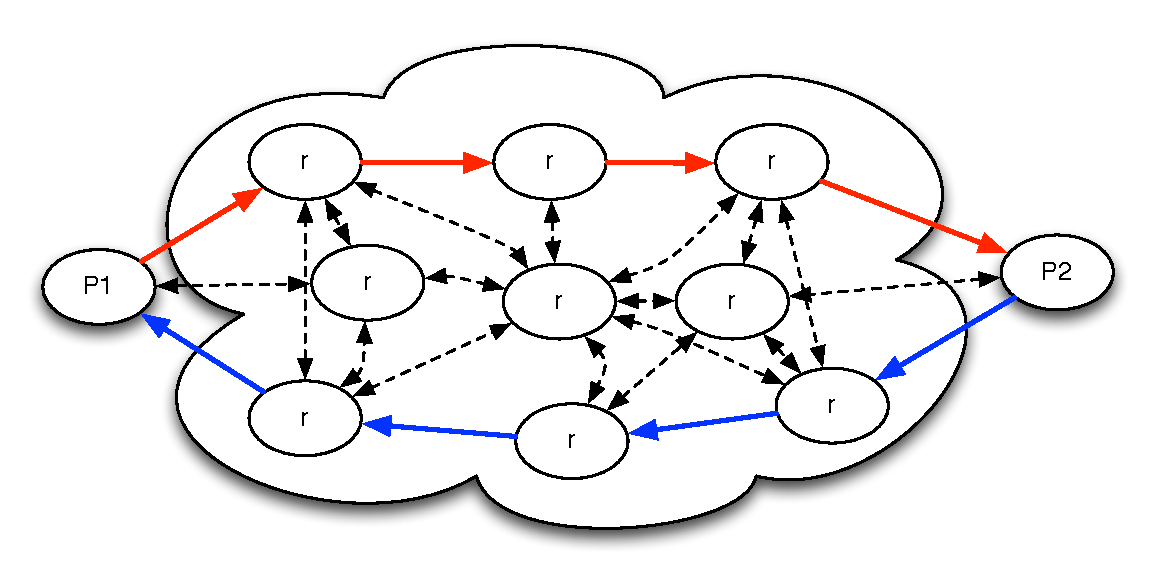
\includegraphics[scale=0.5]{./images/pool.pdf}
\end{center}
\caption{A sample bidirectional circuit configuration in which two parties communicate using mutually exclusive ARs in both directions. Note that it is not required for each circuit to be the same length, nor is it required that the intersection of the routers for each direction of the circuit to be empty (i.e., routers may \emph{unknowingly} support sessions traversing in both directions).}
\label{fig:pool}
\end{figure}

\begin{algorithm}[ht!]
  \caption{Encrypted Interest Generation}
  \begin{algorithmic}[1]
    \Require{Interest $\mathsf{int}$, circuit length $n$, AR pool $\mathcal{R}$}
    \Ensure{Encrypted interest $\overline{\mathsf{int}}_{1}^{n}$}
\State $\overline{\mathsf{int}} = \mathsf{int}$
\For{$i = n$ \textbf{ downto } $1$}
  \State $\mathsf{SIndex}_i := H(\mathsf{session}_i + \mathsf{SIV}_i)$
  \State $\mathsf{SIV}_i = \mathsf{SIV}_i + 1$ (mod $2^{\kappa}$)
  \State $\overline{\mathsf{int}}_i^n = R_i / \mathsf{SIndex}_i / \mathsf{Encrypt}_{E_{k_i}}(\overline{\mathsf{int}}, \mathsf{timestamp})$
\EndFor
\State \Return $\overline{\mathsf{int}}_1^n$
\end{algorithmic}
\label{alg:enc_int_gen}
\end{algorithm}

\begin{algorithm}[ht!]
  \caption{AR Encrypted Interest Forwarding}
  \begin{algorithmic}[1]
    \Require{$\overline{\mathsf{int}}_i^j$}
    \Ensure{$(\overline{\mathsf{int}}_{i+1}^j, \mathsf{session}_i)$ or discarded packet}
\If{$\mathsf{SIndex}_i \in \mathsf{ST}_i$}
  \State Let $(\mathsf{session}_i, E_{k_i}, M_{k_i}, \mathsf{EIV}_i, \mathsf{SIV}_i)$ be the session information associated with $\mathsf{SIndex}_i$
  \State $\mathsf{SIV}_i := \mathsf{SIV}_i + 1$ (mod $2^{\kappa}$)
  \State $\mathsf{SIndex}_i := H(\mathsf{session}_i + \mathsf{SIV}_i)$
  \State Update $(\mathsf{SIndex}_i, \mathsf{session}_i, \mathsf{SIV}_i)$ in the session table $\mathsf{ST}_i$
  \State $(\overline{\mathsf{int}}_{i+1}^{j}, timestamp) := \mathsf{Decrypt}_{E_{k_i}}(\overline{\mathsf{int}}_{i}^{j})$
  \If{decryption fails or $\mathsf{timestamp}$ is not current}
    \State Discard $\overline{\mathsf{int}}_{i}^{j}$
  \Else
    \State Persist tuple $T_i = (\overline{\mathsf{int}}_{i}^{j}, \overline{\mathsf{int}}_{i+1}^{j}, \mathsf{session}_i)$ to pending interest table $\mathsf{PT}_i$
    \State \Return $(\overline{\mathsf{int}}_{i+1}^{j}, \mathsf{session}_i)$
  \EndIf
\Else
  \State Discard $\overline{\mathsf{int}}_{i}^{j}$ \Comment{Some form of interest flooding prevention should be employed here}
\EndIf
\end{algorithmic}
\label{alg:enc_int_forward}
\end{algorithm}

\begin{algorithm}[ht!]
  \caption{AR Content Handling}
  \begin{algorithmic}[1]
    \Require{Content $\overline{data_{i+1}^j}$ in response to interest $\overline{\mathsf{int}}_{i+1}^{j}$}
    \Ensure{Encrypted data packet $data_{i}^j$}
\State Recover tuple $T_i = (\overline{\mathsf{int}}_{i}^{j}, \overline{\mathsf{int}}_{i+1}^{j}, \mathsf{session}_i)$ based on $data_{i+1}^j$
\State Parse $\overline{data_{i+1}^j}$ as a tuple $(data_{i+1}^j, \sigma_{i+1})$
\If{$\sigma_{i+1} = \epsilon$ and $M_{k_{i+1}} = \epsilon$} \Comment{Last hop router - does not verify MAC}
  \State Pass
\ElsIf{$\sigma_{i+1} \not= \epsilon$ and $M_{k_{i+1}} \not= \epsilon$}
  \If{$\sigma_{i+1} = \mathsf{Verify}_{M_{k_{i+1}}}(data_{i+1}^j)$}
    \State Pass
  \Else
    \State \Return $\mathsf{Error}$ \Comment{MAC verification did not pass}
  \EndIf
\Else \Comment{There was either a tag or we don't have the upstream MAC key - either way, we error}
  \State \Return $\mathsf{Error}$
\EndIf

\State Remove signature and name from $data_{i+1}^j$    
\State Create new empty data packet $data_i^j$
\State Set name on $data_i^j$ as the name on $\overline{\mathsf{int}}_{i}^{j}$
\State $data_i^j := \mathsf{Encrypt}_{E_{k_i}}(data_i^j)$
\State $\sigma_i := \mathsf{MAC}(data_i^j)$
\State $\overline{data_{i}^j} = ((data_i^j, \sigma_i))$
\State \Return $\overline{data_{i}^j}$

\end{algorithmic}
\label{alg:ar_content_handler}
\end{algorithm}

\begin{figure}[ht!]
\begin{center}
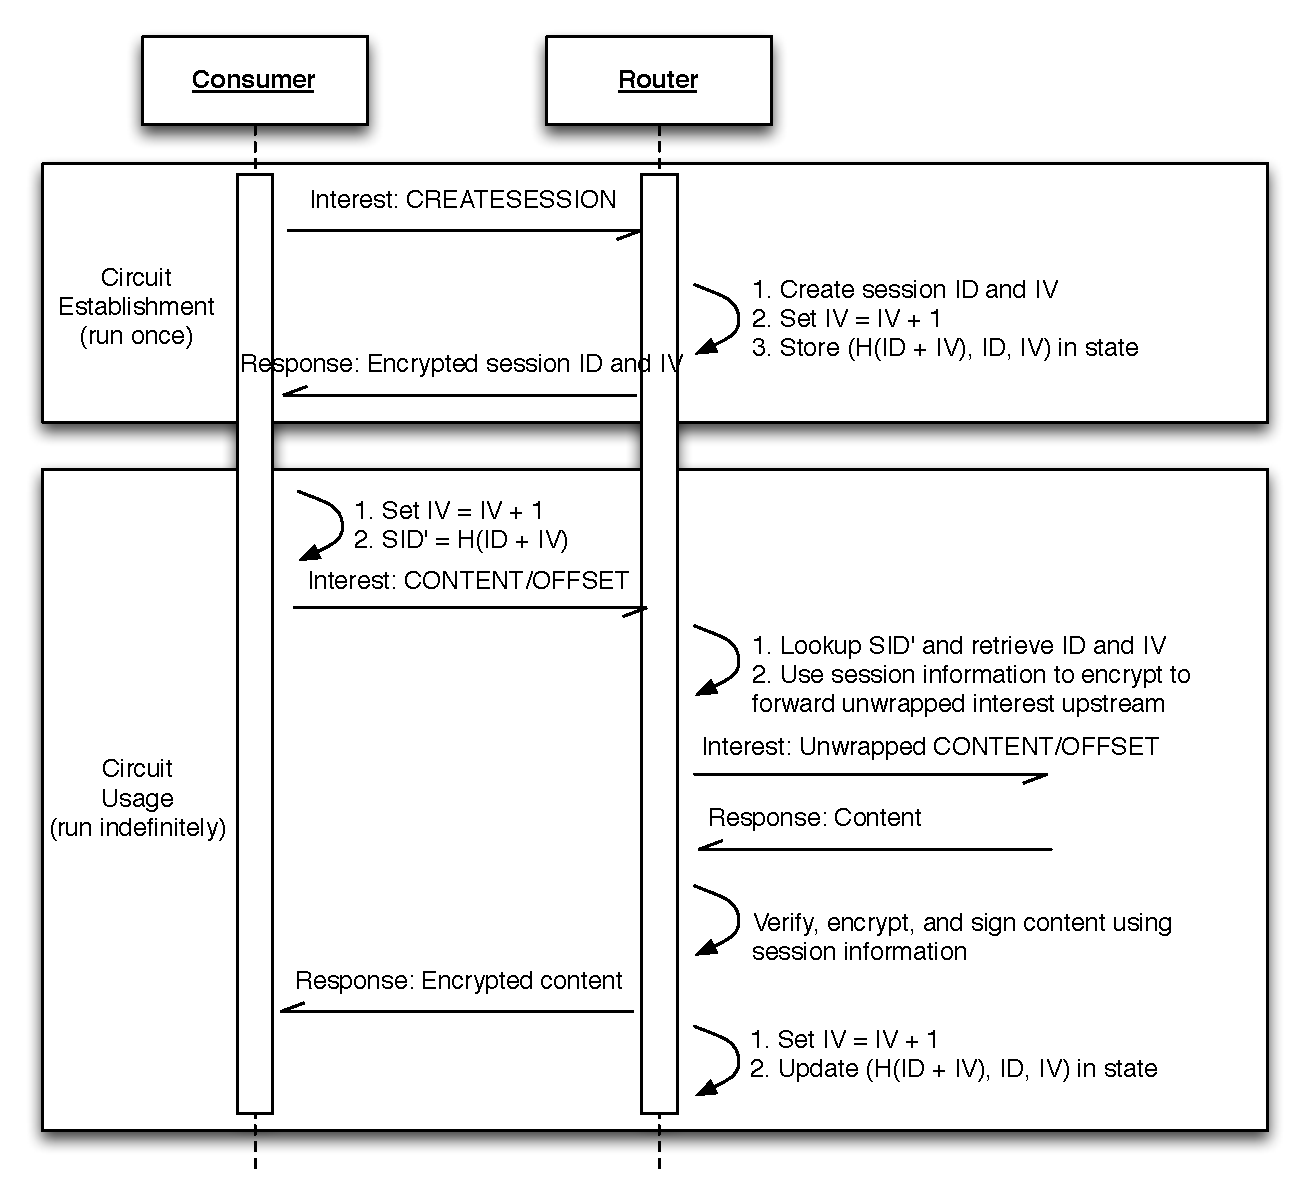
\includegraphics[scale=0.65]{./images/circuit_usage.pdf}
\end{center}
\caption{Visual depiction of the interaction between the consumer and the first hop router. The procedure repeats in the same manner for all further upstream routers after each interest is unrolled and resulting content is encrypted.}
\label{fig:circuit_usage}
\end{figure}

\section{Instantiating Cryptographic Primitives}
Given the generic design presented in the above section, we now need to consider exactly which cryptographic primitives will be used to instantiate this design in usable software. Observe that we require the following primitives:
\begin{enumerate}
  \item CCA-secure symmetric key encryption scheme $\Pi_E = (\mathsf{Gen}_E, \mathsf{Encrypt}, \mathsf{Decrypt})$ (content encryption and decryption.
  \item Arbitrary input and output collision resistant hash function $H$ (content signing and session identification).
  \item CMA-EF secure message authentication code (MAC) scheme $\Pi_M = (\mathsf{Gen}_M, \mathsf{Mac}, \mathsf{Verify})$ and (content signing)
\end{enumerate}

% Following the design of the original {\sf AND\=aNA}, we will use asymmetric encryption with RSA-OAEP. For efficiency reasons, we will use hybrid encryption (i.e., use asymmetric encryption to protect symmetric keys for more efficient encryption and decryption) with AES-GCM, as opposed to AES-HMAC which is used in the preliminary {\sf AND\=aNA} design. \footnote{{\sf AND\=aNA} uses the OpenSSL implementation of AES-HMAC, which uses SHA-1 as the fixed-length hash function for the HMAC.} 

AES-GCM will be used as the CCA-secure symmetric key encryption scheme $\Pi_E$, the Keccak hash function will be used for the arbitrary length input and fixed-length (256-bit) output hash function $H$, and the highly efficient SipHash PRF (as a CMA-EF secure MAC) will serve as the basis for the MAC scheme $\Pi_M$.

With these particular cryptographic primitive instantiations, we now analyze the performance bottlenecks of the {\sf AND\=aNA-v2} design. We do so on a case-by-case basis below, noting optimizations that can be implemented in the design along the way.
\begin{description}
  \item[Content encryption:] AES-GCM operates in counter-mode for CPA-secure encryption and uses the GHASH hash function, based on finite field operations in $GF(2^{128})$, to generate a tag based on the corresponding ciphertext. For efficiency reasons, the ``key stream'' of the block cipher can be precomputed prior to the arrival of content, or, alternatively, while an interest is being handled upstream (see Figure \ref{fig:circuit}), meaning that the ciphertext and tag generation complexity for a ciphertext of $n$ 128-bit blocks reduces to $n$ XOR operations and $n$ GHASH computations. Clearly, the GHASH computation dominates this complexity, and thus the efficiency of content encryption reduces to highly efficient multiplcation in $GF(2^{128})$. 
  \item[Session identification:] Computing session identifiers (that are sent in the clear) require a single modular addition and hash function invocation. Clearly, the efficiency of the Keccak hash function dominates in this regard.
  \item[Interest encryption:] Interest encryption will be done using AES-GCM with the same content encryption key. As such, with pre-computed key streams (i.e., encryptions of the counter values) done at each router, the efficiency of this step reduces to the efficiency of the GHASH function. \footnote{The design can easily be amended to use a different symmetric key and counter IV for interest and content encryption.}
  \item[Content signature generation/verification:] The complexity of both of these procedures is clearly dominated by the efficiency of the Keccak hash function. Symmetric MAC tag generation and verification are far more efficient than the Keccak hash function.
\end{description}

\begin{figure}[ht!]
\begin{center}
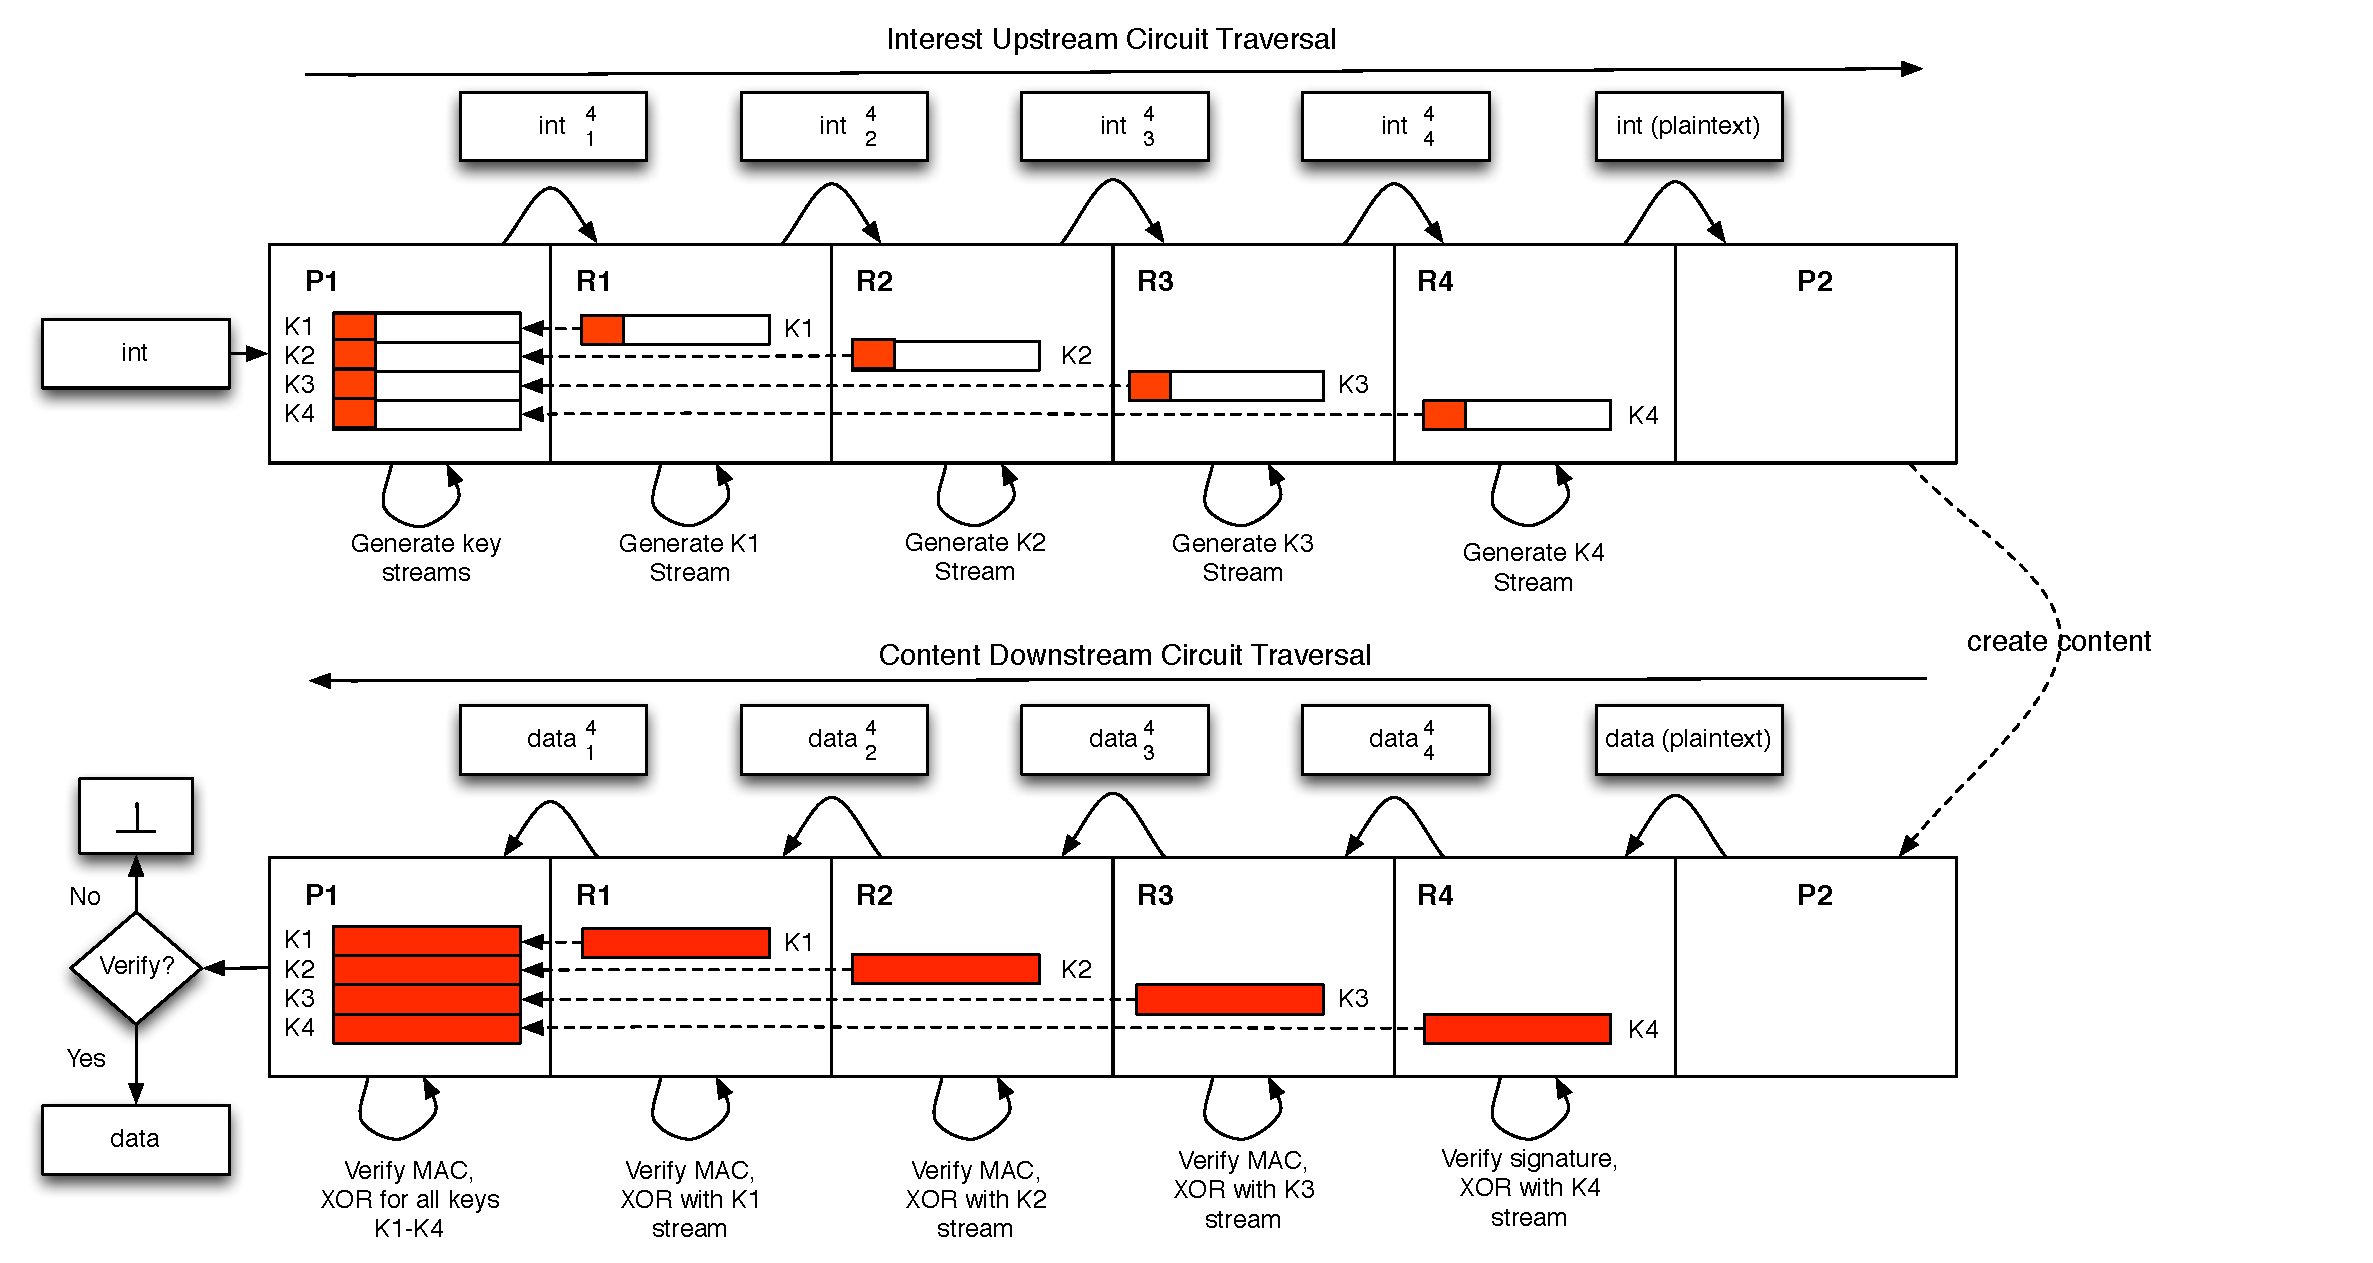
\includegraphics[scale=0.45]{./images/ctr_split.pdf}
\end{center}
\caption{Visual depiction of keystream precomputation during upstream interest traversal and the resulting half of AES-GCM that must be computed for the resulting content flowing downstream. We again emphasize that keystream ``pumping'' for AES-GCM can be done for interests as well.}
\label{fig:circuit}
\end{figure}

We now evaluate these cryptographic algorithms with respect to their performance. Although the performance of all of the proposed cryptographic algorithms are well studied in the literature, we performed our own experiemental analysis that uses the same baseline machine for the benchmarking. Tables \ref{tab:baseline} and \ref{tab:our-baseline} detail these relevant performance metrics (in terms of cycles/byte for each piece of input) to establish a sense of the relative computational complexity of each algorithm.

\begin{table}
\centering
\caption{Published performance measurements for the cryptographic algorithms to be used in the implementation of {\sf AND\=aNA-v2}. AES performance on Intel processors is far superior to other block ciphers with the AES-NI instruction set. We also note that it was not our intention to find a set of performance measurements for each algorithm on the same machine. The data in this table simply serves as a reference to the relative difference in cost for each algorithm.}
\label{tab:baseline}
  \begin{tabular}{| c | c | c |} \hline
  Primitive & Platform/Specifications & Cycles/Byte \\ \hline
  AES-GCM \cite{aesgcm-intel}         & Sandy Bridge & 2.53 \\
  AES-GCM \cite{aesgcm-intel}         & Haswell & 1.03 \\
  AES-GCM \cite{aesgcm-intel}         & i7-2600K Processor (no AES-NI$^*$) & 10.42 \\
  AES-HMAC \cite{aesgcm-intel}        & Sandy Bridge & 6.14 \\
  AES-HMAC \cite{aesgcm-intel}        & Haswell & 4.71  \\
  GHASH \cite{aesgcm-intel}           & Sandy Bridge & 1.79  \\
  GHASH \cite{aesgcm-intel}           & Haswell & 0.40  \\
  HMAC                                & * & *  \\
  SHA-256 \cite{nist-sha3}            & i3-2310M; h6sandy; supercop-20120521  & 17.25 \\
  Keccak-256 \cite{nist-sha3}         & i3-2310M; h6sandy; supercop-20120521  & 10.25  \\
  SipHash-2-4 (long messages) \footnote{The integer parameters $c$ and $d$ in SipHash-$c$-$d$ denote the number of compression and finalization rounds, respectively.} \cite{siphash} & amd64 64-bit & 1.95 \\ 
  SipHash-2-4 (long messages) \cite{siphash}      & i3-2310M; Sandy Bridge (206a7)  & 2.98 \\ \hline
  % RSA-OAEP                            & * & * \\ \hline
  \end{tabular}
\end{table}

\begin{table}
\centering
\caption{Cryptographic algorithm performance measurements based on the current (i.e., latest stable release) OpenSSL implementation. All metrics were captured on a system running Ubuntu 13.04 32-bit with an Intel Core i7-3770 CPU (@ 3.4Ghz x 8) with 16GB DDR3 memory.}
\label{tab:our-baseline}
  \begin{tabular}{|c | c |} \hline
  Primitive  & Cycles/Byte \\ \hline
  AES-128 (256 size blocks)     & 192.58 \\ % 17655042.14 \\ % 1649643, 2.99 \\
  AES-128 (1024 size blocks)    & 189.94 \\ % 17900456.38 \\ %416745, 2.98 \\
  GHASH (256 size blocks)      & 15.62 \\ % 217673236.12 \\ %20338843, 2.99 \\
  GHASH (1024 size blocks)     & 15.17 \\ % 224086817.40 \\ %5234528, 2.99 \\
  HMAC (256 size blocks)       &  75.659 \\ % 44938477.60 \\ % 4198939, 2.99 \\
  HMAC (1024 size blocks)       & 47.2947 \\ % 71889723.08 \\ % 1679299, 2.99 \\
  SHA-256 (256 size blocks)     & 146.727 \\ % 23172345.15 \\ % 2165166, 2.99 \\
  SHA-256 (1024 size blocks)    & 119.738 \\ % 28395280.27 \\ % 663296, 2.99 \\
  Keccak-256 (256 size blocks) & 42720.00 \\
  Keccak-256 (1024 size blocks) & 192362.00 \\
  SipHash-2-4 (256-bit messages) & 1.65 \\ % 256 tests passed in 0.189ms, 0ns per test
  SipHash-2-4 (1024-bit messages) & 1.78 \\ \hline % 1024 tests passed in 6.866ms, 0ns per test
  % RSA-OAEP (public) (2048-bit modulus)  & 1701.91 \\ % 77803, 9.97 \\ \hline
  % RSA-OAEP (private) (2048-bit modulus)  & 54068.6 \\ \hline % 2449, 9.97 \\ \hline
  \end{tabular}
\end{table}

As expected, the block ciphers and SipHash PRF are the highest performing algorithms used in the design of {\sf AND\=aNA-v2}, especially with platform-specific instructions available for such cryptographic procedures. We note that due to our splitting in the AES-CTR encryption and GHASH computation for generating the content ciphertext and corresponding tag, we need only really consider the performance of the GHASH function, shown below.

\begin{align*}
X_i = 
\left\{
  \begin{array}{ll}
    0  & \mbox{for } i = 0 \\
    (X_{i-1} \oplus A_i) \cdot H  & \mbox{for } i = 1,\dots,m-1 \\
    (X_{m-1} \oplus (A_m^* || 0^{128 - v})) \cdot H  & \mbox{for } i = m \\
    (X_{i-1} \oplus C_{i-m}) \cdot H  & \mbox{for } i = m+1,\dots,m+n-1 \\
    (X_{m+n-1} \oplus (C_n^* || 0^{128 - u})) \cdot H  & \mbox{for } i = m+n \\
    (X_{m+n} \oplus (\mathsf{len}(A) || \mathsf{len}(C)))\cdot H  & \mbox{for } i = m+n+1 
  \end{array}
\right.
\end{align*}

Note that all multiplication $\cdot$ is done over polynomials in $GF(2^{128})$, where $H$ is the ciphertext corresponding to the plaintext $0^n$. In our design there will be no additional authenticate data (AAD); perhaps the session identifier could be used, but we do not require nor enforce any AAD. Fortunately, there exists numerous techniques to speed up the performance of this procedure, including carry-less Karatsuba multiplication and (deferred) polynomial reduction via the ``Montgomery'' technique \cite{aesgcm-intel}. Collectively, it is clear that performance of the GHASH computation is expected to exceed performance of HMAC(-SHA-1). 

As for the Keccak hash function, we do not expect to achieve any significant performance improvements beyond what is already presented in the literature. We will use the optimized implementation provided by the authors in the SHA-3 competition \cite{keccak-files}. Similarly, due to the high performance of the optimized SipHash procedure, we will not explore any additional optimizations for this algorithm.

% \todo[inline]{FINISH THIS!}

\section{Preliminary Performance Evaluation and Cost Models}
In order to justfiy {\sf AND\=aNA-v2} as an alternative to existing solutions for low-latency, bidirectional traffic over NDN, we must first establish a baseline of performance metrics against which we can compare our design. Since the original version of {\sf AND\=aNA} targeted circuits of length $2$ (i.e., with two ARs), we focus on the same length circuits in these experiments. We note that there is nothing restricting us from lifting this constraint in future experiments. In order to adequately determine a baseline of performance metrics, we instantiated two parties (both acting as a data producer and consumer) interacting by requesting moderately-sized content in short, frequent intervals. In order ensure that such content is never satisfied by the cache of an intervening AR, which is a reasonable assumption for real-time voice and video applications that always want fresh content instead of stale cached content, each piece of content is requested from an anonymized namespace and indexed by a sequence number. For example, if the two parties $P_1$ and $P_2$ are communicating and $P_1$ wants to request the latest content from $P_2$, it will issue an (encrypted)interest to {\tt ccnx:/$P_2$/$S$}, where $S$ is the sequence number that is incremeneted as soon as the interest is issued. This ensures that such interests are never satisfied by the content in an AR cache throughout the duration of the session. 

With this type of traffic generation application, we then tested its performance under the following scenarios:
\begin{enumerate}
  \item $P_1$ and $P_2$ are connected point-to-point (i.e., no hops).
  \item $P_1$ and $P_2$ are connected through two ``insecure'' ARs that perform no interest or content encryption (i.e., each AR just serves as an application-level proxy to forward interests and content along through the circuit).
  \item $P_1$ and $P_2$ are connected through two ``secure'' ARs that perform interest and content encryption as per the {\sf AND\=aNA} design.
\end{enumerate}
Table \ref{tab:baseline} shows the performance results from such scenarios 1, 2, and 3, in which performance is characterized as the end-user latency between issuing an interest and receiving the intended content. In this case, we refer to the performance in terms of latency, where $L_i$ denote the average latency and $\sigma_i$ denote its standard deviation for party $i$ ($i \in \{1,2\}$). All experiments were collected using the following methdology:
\begin{itemize}
  \item Each party generates 1000 traffic according to an uniform distribution with $pmf = 1/100$. 
  \item Each party responds to all interests with a random blob of 150 bytes. \footnote{This value was chosen to match the average size of a Skype video call packet. Are experiments with different size pieces of content warranted for this proof of concept?}
\end{itemize}

\begin{table}
\centering
\caption{Baseline performance metrics gathered from the three scenarios discussed in the text.}
\label{tab:baseline}
  \begin{tabular}{|c || c c | c c|} \hline
  Scenario & $L_1$ & $\sigma_1$ & $L_2$ & $\sigma_2$ \\ \hline
  1 & $0.00735$ & $0.00798$ & $0.00340$ & $0.00053$ \\
  2 & $0.01905$ & $0.13791$ & $0.02248$ & $0.13923$ \\
  3 & $0.01321$ & $0.00257$ & $0.01359$ & $0.00567$ \\ \hline
  \end{tabular}
\end{table}

According to the preliminary experimental evaluation, it appears as though low-latency, bidirectional communication is realtively feasible with the current {\sf AND\=aNA} design. However, we would like to do better. To that end, we first formally capture the performance of the {\sf AND\=aNA} (symmetric variant) and {\sf AND\=aNA-v2} designs to enable quantitative comparison using the concrete cryptographic primitives discussed in the previous following section. First, let $T_1^{\mathsf{S}}$ and $T_2^{\mathsf{A}}$ be the expected total time required to retrieve one piece of content in the symmetric {\sf AND\=aNA} and asymmetric {\sf AND\=aNA-v2} designs, respectively. Assume that a circuit consists of $n$ ARs, all encrypted interests consist of a single 128-bit block, and all respective content packets consist of $b$ 128-bit blocks. Finally, let $T_{\mathsf{AES}}$, $T_{\mathsf{HMAC}}$, $T_{\mathsf{GHASH}}$, $T_{\mathsf{RSA}}$, $T_{\mathsf{MAC}}$, and $T_{\mathsf{HASH}}$ denote the time required to perform AES, HMAC, GHASH, RSA, MAC, and an arbitrary hash function computation, respectively. Note that we separate the time required to encrypt a single block of plaintext with AES from the corresponding MAC scheme (i.e., HMAC or GHASH) for notational convenience. We also introduce the additional quantities $H_1 = \sum_{i=0}^{n-1}i$ and $H_b = \sum_{i=0}^{n-1}(b + i)$, which will be used to count the blocks of ciphertext that are accumulated as interests and content flow upstream and downstream. We now present the expressions for $T_1^{\mathsf{S}}$ and $T_2^{\mathsf{A}}$ as follows:

%%% In both, Hash of content increases by 1 since each ciphertext includes a new single block tag, encryption is just remasking the same set of bits over and over again, so the ciphertext never grows in size this way (i.e. ciphertext from upstream serves as plaintext for the downstream)
\begin{align*}
T_1^{\mathsf{S}} & = \underbrace{2n(T_{\mathsf{AES}} + T_{\mathsf{HMAC}}) }_{\text{interests}} + \underbrace{2nb(T_{\mathsf{AES}} + T_{\mathsf{HMAC}}) }_{\text{content encryption}} + \underbrace{2T_{\mathsf{HASH}}\left(nb + \frac{n(n+1)}{2}\right) + 2nT_{\mathsf{RSA}}}_{\text{sign/verify}}  %nb cost for hash at each AR and signer (ciphertext doesn't accumulate)
\end{align*}

\begin{align*}
T_2^{\mathsf{A}} & = \underbrace{2n(T_{\mathsf{HASH}} + T_{\mathsf{AES}} + T_{\mathsf{GHASH}}) }_{\text{interest encr/decr}} + \underbrace{2n(b+1)T_{\mathsf{GHASH}} }_{\text{content encr/decr}} + \underbrace{2T_{\mathsf{HASH}}\left(nb + \frac{n(n+1)}{2}\right) + 2nT_{\mathsf{MAC}}}_{\text{sign/verify}}
\end{align*}

It is important to emphasize that we are comparing the symmetric variant of {\sf AND\=aNA} with the asymmetric variant of {\sf AND\=aNA-v2}. As stated in \cite{andana}, the symmetric variant does not enjoy consumer and producer unlinkability since session identifiers are sent in cleartext. However, for the sake of comparing performance, we opted to compare the \emph{best} version of {\sf AND\=aNA} with the \emph{worst} variant of {\sf AND\=aNA-v2}. Accordingly, comparing the performance of these two seemingly uncompatible designs will serve to intensify the improvement of the {\sf AND\=aNA-v2} design both in terms of performance (for this particular use case) and security/anonymity. 
As one can see, $T_1^{\mathsf{S}}$ and $T_2^{\mathsf{A}}$ are quite different. While content signature generation seemingly consumes the majority of the computation in the {\sf AND\=aNA} design, the {\sf AND\=aNA-v2} design enjoys highly efficient content signature generation by using symmetric MACs. Since adjacent ARs in the circuit share a common MAC key that is established during the circuit and session establishment protocol, a MAC can effectively remove the need for an expensive hash computation (on possibly large messages) and subsequent signature. Furthermore, there are no asmmetric cryptographic operations needed for this new design, which intuitively means that it will achieve better performance. Of course, we require empirical evidence to support this claim, and the implementation and evaluation of {\sf AND\=aNA-v2} will provide exactly that information.

% In contrast to content signature generation, interest encryption is clearly more expensive in {\sf AND\=aNA-v2}. However, we note that all PKI operations are done on a single symmetric 128-bit key, which is then later used to encrypt the interest, session identifier, and timestamp as per Algorithm \ref{alg:enc_int_gen}. Therefore, even though a single asymmetric encryption and decryption procedures are performed for each AR in the circuit, it may still be the case that the input to such operations is \emph{smaller} than the size of content being hashed and signed in {\sf AND\=aNA}. based on these observations, for applications where content is relatively large, we expect that $T_2^{\mathsf{A}}$ will subsume $T_1^{\mathsf{S}}$ in all scenarios. Of course, we require empirical evidence to support this claim, and the implementation and evaluation of {\sf AND\=aNA-v2} will provide exactly that information.

% \todo[inline]{Discuss the rationale here... as well as the means of how to compare them...}

% \begin{itemize}
%   \item counter mode and precomputation of key stream (or at least, in paralllel), and thus super fast encryption
%   \item optional: use AES-GCM for authenticated encryption of content (CCA security too?)
%   \item optional signature verification
%   \item QUICK signature generation using MACs
% \end{itemize}

\section{Correctness and Security Analysis}
In order to assess the security of {\sf AND\=aNA-v2} it is important to first define an adversarial model and corresponding definition of security. To this end, we define an adversarial model for {\sf AND\=aNA-v2} that has the same capabilities as presented in \cite{andana}:
\begin{itemize}
	\item Deploy compromised routers
	\item Compromise existing routers
	\item Control content producers
	\item Deploy compromised caches
	\item Observe and replay traffic
\end{itemize}
Furthermore, any of these actions or capabiltiies can be carried out adaptively (i.e., in response to status updates from the network or based on the adversary's observations). We also note that the time required to carry out an attack is non-negligibly larger than the average RTT for an interest-content exchange in order to make this model realistic. 

We also make use of the same notions of producer and consumer anonymity and unlinkability to define the security of this scheme. Before reintroducing these definitions, we first establish the relevant notation. An adversary $\mathcal{A}$ is defined as a 4-tuple $(\mathsf{P}_{\mathcal{A}}, \mathsf{C}_{\mathcal{A}}, \mathsf{R}_{\mathcal{A}}, \mathsf{IF}_{\mathcal{A}})$, where each individual component denotes the set of producers, consumers, routers, and interfaces compromised by $\mathcal{A}$, respectively. Following \cite{andana}, a router $r$ is deemed compromised (i.e., $r \in \mathcal{R}_{\mathcal{A}}$) if all of its interfaces belong to $\mathsf{IF}_{\mathcal{A}}$. Similarly, if $\mathcal{A}$ controls a producer or consumer then they have complete (and adaptive) control over how they behave in the application session, meaning that $\mathcal{A}$ can control everything from the timing, format, and actual information of each piece of content. We also define the anonmity set with respect to an interface $\mathsf{if}_i^r$ (i.e., interface $i$ of router $r$) to be 
\begin{align*}
\mathsf{AS}_{\mathsf{if}_{i}^{r}} = \{d | \Pr[d \to_\mathsf{int} r | \mathsf{int} \to \mathsf{if}_i^r] > 0 \},
\end{align*}
and the anonymity set with respect to the adversary $\mathcal{A}$ to be
\begin{align*}
\mathsf{AS}_{\mathcal{A}}^{\mathsf{int}} = \bigcap_{\mathsf{path}^{\mathsf{int}} \cap \mathsf{IF}_{\mathcal{A}}} \mathsf{AS}_{\mathsf{if}_{i}^{r}},
\end{align*}
where $\mathsf{path}^{\mathsf{int}}$ is the set of interfaces along which the interest $\mathsf{int}$ traversed in the circuit from the consumer to the producer. 

Finally, we denote the ``state'' of a network, or configuration, as a snapshot in time of its current activity. Accordingly, each configuration is a relation that maps parties to their actions (e.g., interest or content creation). For circuits of length $n$, let a configuration $C$ be defined as
\begin{align*}
C : \mathsf{C} \to \{(r_1,\dots,r_n,p,\overline{\mathsf{int}}_1^n)\},
\end{align*}
where the $(n + 2)$-element tuple $(r_1,\dots,r_n,p,\mathsf{int}_1^n) \in \mathsf{R}^n \times \mathsf{P} \times \{0,1\}^*$. This relation can be viewed as a map from a consumer $c \in \mathsf{C}$ to a set of routers defining the circuit from $c$ to all producers $p \in \mathsf{P}$ along which interests $\overline{\mathsf{int}}_1^n$ traverse. 

Following in the footsteps of \cite{andana}, we define the security of our design in the context of indistinguishable network configurations. Specifically, two configurations $C$ and $C'$ are said to be \emph{indistinguishable with respect to $\mathcal{A}$}, denoted $C \equiv_{\mathcal{A}} C'$, if for all such polynomial-time adversaries $\mathcal{A}$ there exists a negligible function $\epsilon$ such that 
\begin{align*}
\left|\Pr[\mathcal{A}(1^n, C) = 1] - \Pr[\mathcal{A}(1^n, C') = 1]\right| \leq \epsilon(\kappa),
\end{align*}
for the global security parameter $\kappa$.

We now define security of our design in terms of consumer and producer anonymity and unlinkability. These can be found in \cite{andana}, but we provide them here for completeness. We also provide new definitions that make sense in the context of the bidirectional session case that {\sf AND\=aNA-v2} is intended to support.
\begin{defn}
\cite{andana} For $u \in (\mathsf{C} \setminus \mathsf{C}_{\mathcal{A}})$, $u$ is said to have {\sf consumer anonymity} in configuration $C$ with respect to adversary $\mathcal{A}$ if there exists $C' \equiv_{\mathcal{A}} C$ such that $C'(u') = C(u)$ and $u' \not= u$. 
\end{defn}
\begin{defn}
\cite{andana} Given $\overline{\mathsf{int}}_1^n$ and $p \in \mathsf{P}$, $u \in \mathsf{C}$ has {\sf producer anonymity} in configuration $C$ with respect to $p$ and adversary $\mathcal{A}$ if there exists a configuration $C' \equiv_{\mathcal{A}} C$ such that $\overline{\mathsf{int}}_1^n$ is sent by a non-compromised consumer to a producer different from $p$. 
\end{defn}
\begin{defn}
Two entities $u_1$ and $u_2$, both serving as producer and consumer of content in an application session, are said to have {\sf session anonymity} in configuration $C$ with respect to adversary $\mathcal{A}$ if both $u_1$ and $u_2$ enjoy producer and consumer anonymity in $C$ with respect to $\mathcal{A}$.
\end{defn}
\begin{defn}
\cite{andana} We say that $u \in (\mathsf{C} \setminus \mathsf{C}_{\mathcal{A}})$ and $p \in \mathsf{P}$ are {\sf unlinkable} in $C$ with respect to an adversary $\mathcal{A}$ if there exists a configuration $C' \equiv_{\mathcal{A}} C$ where $u$'s interests are sent to a producer $p' \not= p$.
\end{defn}

We emphasize that the fundamental differences between the design of {\sf AND\=aNA} and {\sf AND\=aNA-v2} are that, in {\sf AND\=aNA-v2}, each adjacent router will share a private MAC key used for efficient content signature generation (and, optionally, verification) and sessions are identified by the output of $H$ (rather than encrypting and decrypting interests using expensive asymmetric procedures). Accordingly, the proofs of anonymity and privacy need to be augmented to take this into account. The remainder of the design is syntactically equivalent to that of {\sf AND\=aNA}, and so we may restate the theoreoms without proof. However, in doing so, we generalize them to circuits of length $n \geq 2$. 

\begin{thm}
Consumer $u \in (\mathsf{C} \setminus \mathsf{C}_{\mathcal{A}})$ has consumer anonymity in configuration $C$ with respect to adversary $\mathcal{A}$ if there exists $u \not= u'$ such that any of the following conditions hold:
\begin{enumerate}
	\item $u, u' \in \mathsf{AS}_{\mathcal{A}}^{C_4(u)}$
	\item There exists ARs $r_i$ and $r_i'$ such that $r_i,r_i' \notin \mathsf{R}_{\mathcal{A}}$, both $r_i$ and $r_i'$ are on the circuit traversed by $C_4(u) = \overline{\mathsf{int}}_1^n$.
\end{enumerate}
\end{thm}
\begin{proof}
See \cite{andana}.
\end{proof}

\begin{thm}
Consumer $u$ has producer anonymity in configuration $C$ with respect to producer $p \in \mathsf{P}$ and adversary $\mathcal{A}$ if there exists a pair of ARs $r_i$ and $r_i'$ such that $r_i$ and $r_i'$ (for some uncompromised entity $u \notin \mathsf{C}_{\mathcal{A}}$) are on the path traversed by $C_4(u) = \overline{\mathsf{int}}_1^n$, $C_1(u) = C_1(u')$, and $C_3(u) = p \not= C_3(u')$.
\end{thm}
\begin{proof}
See \cite{andana}.
\end{proof}

\begin{cor}
Consumer $u \in (\mathsf{C} \setminus \mathsf{C}_{\mathcal{A}})$ and producer $p \in \mathsf{P}$ are unlinkable in configuration $C$ with respect to adversary $\mathcal{A}$ if $p$ has producer anonymity with respect to $u$'s interests or $u$ has consumer anonymity and there exists a configuration $C' \equiv_{\mathcal{A}} C$ where $C'(u') = C(u)$ with $u' \not= u$ and $u'$'s interests have a destination different from $p$. 
\end{cor}

In addition to security, we must also be concerned about the correct functioning of each AR supporting a session between two parties. In this context, we (informally) define session correctness as the ability of a consumer to correctly decrypt content that is generated \emph{in response to} its original interest. That is, if a consumer issues an interest, it should be able to correctly decrypt the content that it receives. The following factors impact the correctness of the session:
\begin{enumerate}
  \item Each AR $r_1,\dots,r_n$ on the consumer-to-producer circuit should correctly recover the session identifier associated with the current session. 
  \item The session key streams should only be advanced upon the receipt of an interest corresponding to the consumer who initiated the session or content that is generated from the upstream router (potentially the producer) in the circuit.
\end{enumerate}

The first item is necessary in order for each AR to correctly decrypt interests, encrypt content, and perform content signature generation and verification. The second item is necessary so that all content can be correctly decrypted by the consumer. We claim that, given a CCA-secure public key encryption scheme, the probability that either one of these factors being violated by an adversary $\mathcal{A}$ is negligible. Let $\mathsf{ForgeSession}$ and $\mathsf{KeyJump}$ denote the events corresponding to instances where an adversary creates a ciphertext that maps to a valid session identifier for \emph{some} session currently supported by an AR (i.e., the forged session belongs to the routers session table $\mathsf{ST}$), and the event that an adversary causes the key stream for \emph{some} AR in a consumer-to-producer circuit to fall out of sync with the consumer. By the design of {\sf AND\=aNA-v2}, it should be clear that $\mathsf{KeyJump}$ occurs when $\mathsf{ForgeSession}$ occurs, since the key stream is only advanced upon receipt of an interest, but may also occur when an adversary successfully forges a MAC tag corresponding to the signature of a piece of content from the upstream router (or producer). We denote this latter event as $\mathsf{ContentMacForge}$. With the motivation in place, we now formally analyze the probabilities of these events occuring below. For notational convenience, we assume that each event only occurs as a result of some adversarial action, so we omit this relation in what follows.

\begin{lemma}
For all probabilistic polynomial-time adversaries $\mathcal{A}$, there exists some negligible function $\mathsf{negl}$ such that
\begin{align*}
\Pr[\mathsf{ForgeSession}] \leq \mathsf{negl}(\kappa).
\end{align*}
\end{lemma}
\begin{proof}
By the design of {\sf AND\=aNA-v2}, we know that session identifiers are computed as the output of a collision resistant hash function $H : \{0,1\}^* \to \{0,1\}^{m}$, where $m = \mathsf{poly}(\kappa)$ (i.e. polynomial in the global security parameter). Consequently, forging a session identifier \emph{without} the input to $H$ implies that a collision was found, thus violating collision resistance of $H$. Thus, forging a session is equally hard as finding a collision in $H$, or more formally, $\Pr[\mathsf{Collision}(H) = 1] = \Pr[\mathsf{ForgeSession}]$. By the properties of collision resistance of $H$ which states that $\Pr[\mathsf{Collision}(H) = 1] \leq \mathsf{negl}(\kappa)$ for some negligible function $\mathsf{negl}$, it follows that $\Pr[\mathsf{ForgeSession}] \leq \mathsf{negl}(\kappa)$. 

% TODO: asusme that some session is forged... session identifiers are created from hashing the session ID as per the above design, so a forgery implies a collision in the hash function. If we assume a CRH hash, then forgery implies contradiction, and we're done.
\end{proof}

\begin{lemma}
For all probabilistic polynomial-time adversaries $\mathcal{A}$, there exists some negligible function $\mathsf{negl}$ such that
\begin{align*}
\Pr[\mathsf{ContentMacForge}] \leq \mathsf{negl}(\kappa).
\end{align*}
\end{lemma}
\begin{proof}
By the design of {\sf AND\=aNA-v2}, the MAC scheme $\Pi$ used for content symmetric content signature generation and verification is defined as $\Pi = (\mathsf{Gen}, \mathsf{Mac}, \mathsf{Ver})$, where $\mathsf{Gen}$ generates the secret key $k$ used in the scheme, $\mathsf{Mac}_k(m)$ outputs the MAC tag $t := F_k(m)$ for some pseudorandom function $F$, and $\mathsf{Ver}_k(m, t)$ outputs $1$ if $t = \mathsf{Mac}_k(m)$ and $0$ otherwise. This is known and proven to be a secure MAC scheme [does this warrant citation?], meaning that for all probabilistic polynomial-time adversaries $\mathcal{A}$ there exists a negligible function $\mathsf{negl}$ such that $\Pr[\mathsf{MacForce}_{\mathcal{A},\Pi}(1^{\kappa}) = 1] \leq \mathsf{negl}(\kappa)$, and since $\mathsf{ContentMacForce}$ occurs exactly when the even $\mathsf{MacForce}$ occurs, we have that $\Pr[\mathsf{ContentMacForge}] \leq \mathsf{negl}(\kappa)$.

% TODO: assume secure MAC scheme based on PRF is used, a forgery in the MAC scheme therefore relies on the PRFness of SipHash... If this holds, then ContentMacForge is negligible.
\end{proof}

\begin{lemma}
For all probabilistic polynomial-time adversaries $\mathcal{A}$, there exists some negligible function $\mathsf{negl}$ such that
\begin{align*}
\Pr[\mathsf{KeyJump}] \leq \mathsf{negl}(\kappa).
\end{align*}
\end{lemma}
\begin{proof}
By the design of {\sf AND\=aNA-v2}, it follows that $\Pr[\mathsf{KeyJump}] = \Pr[\mathsf{ForgeSession}] + \Pr[\mathsf{ContentMacForce}]$, and since the sum of two negligible functions is also negligible, it follows that there exists some negligible function $\mathsf{negl}$ such that $\Pr[\mathsf{KeyJump}] \leq \mathsf{negl}(\kappa)$.
\end{proof}

\begin{thm}
Session correctness of {\sf AND\=aNA-v2} is only violated with negligible probability.
\end{thm}
\begin{proof}
This follows immediately from Lemmas 1, 2, and 3 and the fact that the sum of two negligible functions is also negligible.\footnote{This sum comes from the fact that the probability of the ``failure'' events occurring must be taken into account in both directions of the session.} 
\end{proof}

% The primary difference between the design of {\sf AND\=aNA} and {\sf AND\=aNA-v2} is the existence of session state in each AR. In particular, each AR maintains a 

% TODO: sharing sessions does not violate unlinkability as in the original design since they're not sent in cleartext and are independent for each user (by the independence by which keys are chosen), state in theorem and then prove, the implication is that even if they are shared, the attacker cannot force content encryption keys to be used to recover content

% \begin{thm}
% ASD
% \end{thm}
% \begin{proof}
% \end{proof}

% THM: if CCA-secure public key scheme is used, and session IDs (independent) are used to lookup keys for encryption, then the resulting scheme is secure (this is because the session ID determines the key used for CPA-symmetric encryption - AES, so we can think of the session IDs as the keys themselves (just with a layer of indirection) - if keys are independent then session IDs are independent, and sessions determine which keys to use)

% Goal: session keys should not make it easy for an attacker to distinguish between two configurations - they don't (there is a 1-1 correspondence between the session and the keys, so if they could differentiate then they could tell which keys were used apart and could break the security of the encryption scheme - need to prove this formally)
% *** this is the only difference (the shared state between the routers)

% \todo[inline]{Both party anonymity implies both party anonymity...}
% \todo[inline]{Does unlinkability in both directions imply unlinkability of session? Yes...}
% \todo[inline]{See if theorems from \cite{andana} can be mangled to bidirectional case...}

%%%%%%%%%%%%%%%%%%%%%
%%% END MAIN CONTENT
%%%%%%%%%%%%%%%%%%%%%

%%% BIBLIOGRAPHY
\begin{thebibliography}{[MT1]}

\bibitem{voccn} V. Jacobson, D. K. Smetters, N. H. Briggs, M. F. Plass, P. Stewart, J. D. Thornton, and R. L. Braynard. VoCCN: Voice-Over Content-Centric Networks. \emph{In Proceedings of the 2009 Workshop on Re-Architecting the Internet (ReArch '09), ACM, New York, NY, USA} (2009), 1-6. 

\bibitem{andana} S. DiBenedetto, P. Gasti, G. Tsudik, and E. Unzun. {\sf AND\=aNA}: Anonymous named data networking application. \emph{In NDSS '12} (2012).

\bibitem{tor} R. Dingledine, N. Mathewsonn, and P. Syverson. Tor: The Second-Generation Onion Router. \emph{In The 13th USENIX Security Symposium} (2004).

\bibitem{nist-sha3} S. Chang, R. Perlner, W. E. Burr, M. S. Turan, J. M. Kelsey, S. Paul, L. E. Bassham. Third-Round Report of the SHA-3 Cryptographic Hash Algorithm Competition. \emph{National Institute of Standards and Technology (NIST) NISTIR 7896}.

\bibitem{siphash} J. Aumasson and D. J. Bernstein. SipHash: A Fast Short-Input PRF. \emph{Progress in Cryptology - INDOCRYPT 2012, Springer Berlin Heidelberg} (2012), 489-508.

\bibitem{aesgcm-intel} S. Gueron. AES-GCM for Efficient Authenticated Encryption - Ending the Reign of HMAC-SHA-1? \emph{Workshop on Real-World Cryptography, Stanford University, CA} (2013).

\bibitem{attacking-unlinkability} M. Franz, B. Meyer, and A. Pashalidis. Attacking Unlinkability: The Importance of Context. \emph{Privacy Enhancing Technologies. Springer Berlin Heidelberg} (2007).

\bibitem{linkability-attacks} S. Schiffner and S. ClauB. Using Linkability Information to Attack Mix-Based Anonymity Services. \emph{Privacy Enhancing Technologies. Springer Berlin Heidelberg} (2009).

\bibitem{tor-traffic-analysis} S. J. Murdoch and G. Danezis. Low-Cost Traffic Analysis of Tor. \emph{2005 IEEE Symposium on Security and Privacy} (2005).

\bibitem{keccak-files} The Keccak sponge function family. Software and other files. Available online at \url{http://keccak.noekeon.org/files.html}. Last accessed 11/18/13.

% \bibitem{keccak-sw} The Keccak sponge function family. Software performance figures. Available online at \url{http://keccak.noekeon.org/sw_performance.html}. Last accessed 11/18/13.

\end{thebibliography}

\end{document}
